\section{Sección}

\lipsum[1]

\subsection{Algunas cosillas}


\subsubsection{Referencias}

Para referenciar a una palabra del glosario

\glsfirst{JDK} \\
\gls{APK} \\
\gls{JDK} \\
\cite{AngBenNadel}

\subsubsection{Imagen}

\begin{figure}[H]
\centering
  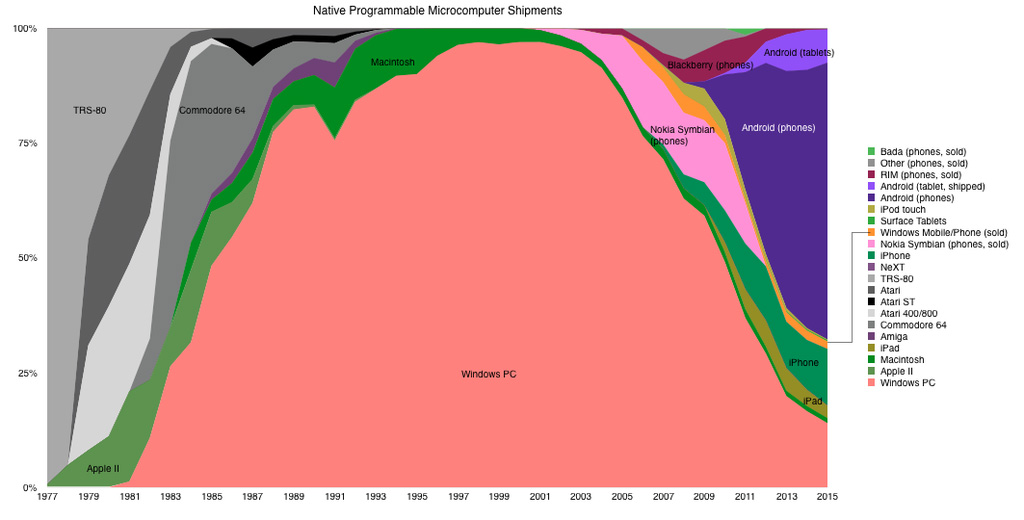
\includegraphics[width=\textwidth]{Figures/ch1/introduction/os_quota}
  \caption{Pie de imagen. }
\end{figure}

\subsubsection{Código}

Bash


\begin{minted}[
frame=lines,
linenos
]{bash}
    cd
    ls
    echo "Hello World"
\end{minted}

Python


\begin{minted}[
frame=lines,
linenos
]{python}
import os
class HelloWorld:
    msg = "Hello World"
    def __init__(self):
        print(self.msg)

if __name__ == '__main__':
    HelloWorld()	
\end{minted}
